% This file was created by tikzplotlib v0.9.8.
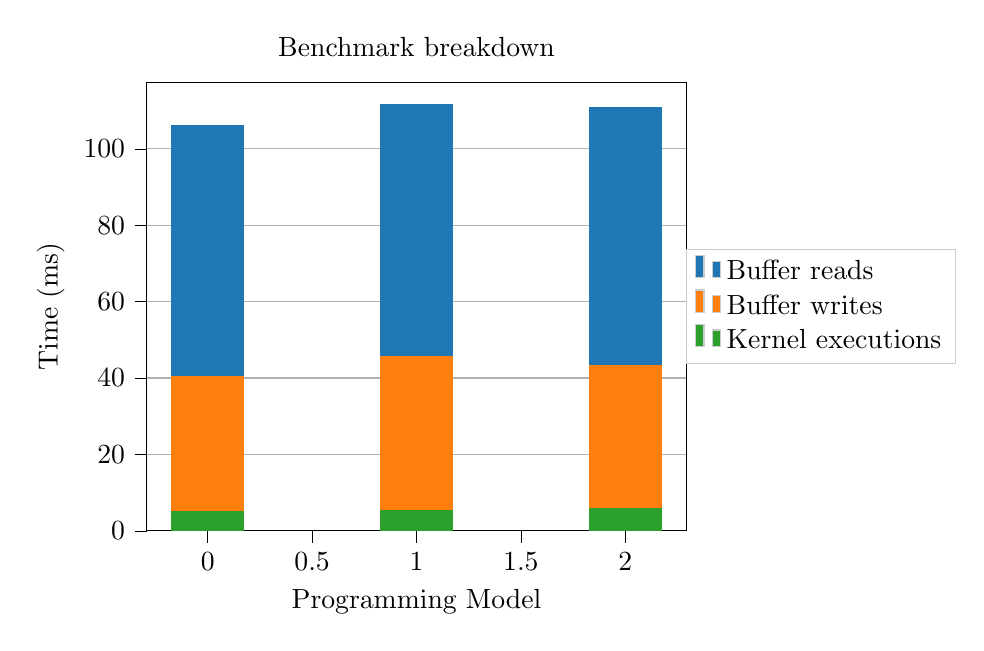
\begin{tikzpicture}

\definecolor{color0}{rgb}{0.12156862745098,0.466666666666667,0.705882352941177}
\definecolor{color1}{rgb}{1,0.498039215686275,0.0549019607843137}
\definecolor{color2}{rgb}{0.172549019607843,0.627450980392157,0.172549019607843}

\begin{axis}[
legend cell align={left},
legend style={
  fill opacity=1,
  draw opacity=1,
  text opacity=1,
  at={(1,0.5)},
  anchor=west,
  draw=white!80!black
},
tick align=outside,
tick pos=left,
title={Benchmark breakdown},
x grid style={white!69.0196078431373!black},
xlabel={Programming Model},
xmin=-0.2925, xmax=2.2925,
xtick style={color=black},
y grid style={white!69.0196078431373!black},
ylabel={Time (ms)},
ymajorgrids,
ymin=0, ymax=117.376884261,
ytick style={color=black}
]
\draw[draw=none,fill=color0] (axis cs:-0.175,40.53220461) rectangle (axis cs:0.175,106.29634618);
\addlegendimage{ybar,ybar legend,draw=none,fill=color0};
\addlegendentry{Buffer reads}

\draw[draw=none,fill=color0] (axis cs:0.825,45.73372929) rectangle (axis cs:1.175,111.78750882);
\draw[draw=none,fill=color0] (axis cs:1.825,43.50616961) rectangle (axis cs:2.175,111.0843118);
\draw[draw=none,fill=color1] (axis cs:-0.175,5.15266011) rectangle (axis cs:0.175,40.53220461);
\addlegendimage{ybar,ybar legend,draw=none,fill=color1};
\addlegendentry{Buffer writes}

\draw[draw=none,fill=color1] (axis cs:0.825,5.45583448) rectangle (axis cs:1.175,45.73372929);
\draw[draw=none,fill=color1] (axis cs:1.825,5.88321827) rectangle (axis cs:2.175,43.50616961);
\draw[draw=none,fill=color2] (axis cs:-0.175,0) rectangle (axis cs:0.175,5.15266011);
\addlegendimage{ybar,ybar legend,draw=none,fill=color2};
\addlegendentry{Kernel executions}

\draw[draw=none,fill=color2] (axis cs:0.825,0) rectangle (axis cs:1.175,5.45583448);
\draw[draw=none,fill=color2] (axis cs:1.825,0) rectangle (axis cs:2.175,5.88321827);
\end{axis}

\end{tikzpicture}
